We validate our implementation with a speed benchmark against competing approaches, and we present the privacy/utility Pareto fronts that can be obtained with GNP networks. 

\subsection{Evaluation of privacy, accuracy and robustness}

For the comparisons, we leverage the DP-SGD implementation from Opacus. We perform a search over a broad range of hyper-parameter values: the configuration is given in Appendix~\ref{app:experiments}. We ignore the privacy loss that may be induced by this hyper-parameter search, which is a limitation per recent studies like~\cite{papernot2022hyperparameter} or~\rebuttal{\cite{ding2022revisiting}}. % The training is performed on a randomly initialized network. %, without data augmentation and without fine-tuning.

\textbf{Accuracy and Privacy.} We validate the performance of our approach on tabular data from Adbench suite~\citep{han2022adbench} using a MLP, and report the result in Table~\ref{tab:tabularutility}. For MNIST (Fig.~\ref{fig:mnistmain} we use a Lipschitz LeNet-like architecture.
 
% On image classification tasks, we benchmark architectures inspired from VGG~\cite{simonyan2014very}, Resnet~\cite{he2016deep} and MLP\_Mixers~\cite{tolstikhin2021mlp}: see appendix for more details. On tabular tasks, we rely on MLP. 


%  Results are reported in Figure~\ref{fig:paretofrontrobust}. We also report in  results on tabular data with a Lipschitz MLP. Networks are trained from scratch, without data-augmentation or pre-training. We leverage the DP-SGD implementation from Opacus and perform a grid search on the hyper-parameters of both methods: the hyper-parameter configuration is given in Appendix~\ref{app:experiments}. We emphasize that the training is performed from scratch on a randomly initialized network, without fine-tuning a foundation model.
% On image classification tasks, we benchmark architectures inspired from VGG~\cite{simonyan2014very}, Resnet~\cite{he2016deep} and MLP\_Mixers~\cite{tolstikhin2021mlp}: see appendix for more details. On tabular tasks, we rely on simple MLP. We ignore the privacy loss that may be induced by hyper-parameter search, which is a limitation per recent studies~\cite{papernot2022hyperparameter}, but is common practice.  

\begin{figure}%[ht]
\centering
\resizebox{0.95\textwidth}{!}{%
  \begin{subfigure}{0.55\textwidth}
        \small
        % \hspace{-0.08\textwidth}
        \begin{tabular}{|p{1cm}>{\raggedleft\arraybackslash}p{0.9cm}>{\raggedleft\arraybackslash}p{0.5cm}>{\raggedright\arraybackslash}p{0.6cm}|cc|}
            \hline
             \multirow{2}{*}{Dataset} & \multirow{2}{*}{Size} & \multirow{2}{*}{Dim.} & \multirow{2}{*}{$\delta$} & \multicolumn{2}{c|}{Validation AUROC $\uparrow$} \\
                     &            &             &          & \makecell{DP-SGD} & \makecell{Clipless\\ DP-SGD} \\
            \hline
            \hline
    ALOI & 39,627 & 27 & $10^{-5}$ & $\textbf{56.5}$ & $56.2$\\
    campaign & 32,950 & 62 & $10^{-5}$ & $\textbf{90.0}$ & $82.2$\\
    celeba & 162,079 & 39 & $10^{-6}$ & $\textbf{96.6}$ & $96.5$\\
    census & 239,428 & 500 & $10^{-6}$ & $\textbf{93.3}$ & $92.5$\\
    donors & 495,460 & 10 & $10^{-6}$ & $\textbf{100.0}$ & $\textbf{100.0}$\\
    magic & 15,216 & 10 & $10^{-5}$ & $\textbf{90.7}$ & $89.7$\\
    shuttle & 39,277 & 9 & $10^{-5}$ & $98.3$ & $\textbf{99.4}$\\
    skin & 196,045 & 3 & $10^{-6}$ & $\textbf{100.0}$ & $99.8$\\
    yeast & 1,187 & 8 & $10^{-4}$ & $66.8$ & $\textbf{75.1}$\\
            \hline
    \end{tabular}
    \caption{\textbf{Best AUROC values (in \%) for models trained under \DP privacy with $\epsilon=1$}, on binary classification tasks of tabular data from Adbench datasets~\cite{han2022adbench}. We use a random stratified split into train (80\%) / validation (20\%).}
    \label{tab:tabularutility}
    \end{subfigure}
    \hspace{0.05\textwidth}
    \begin{subfigure}{0.45\textwidth}
        \centering
        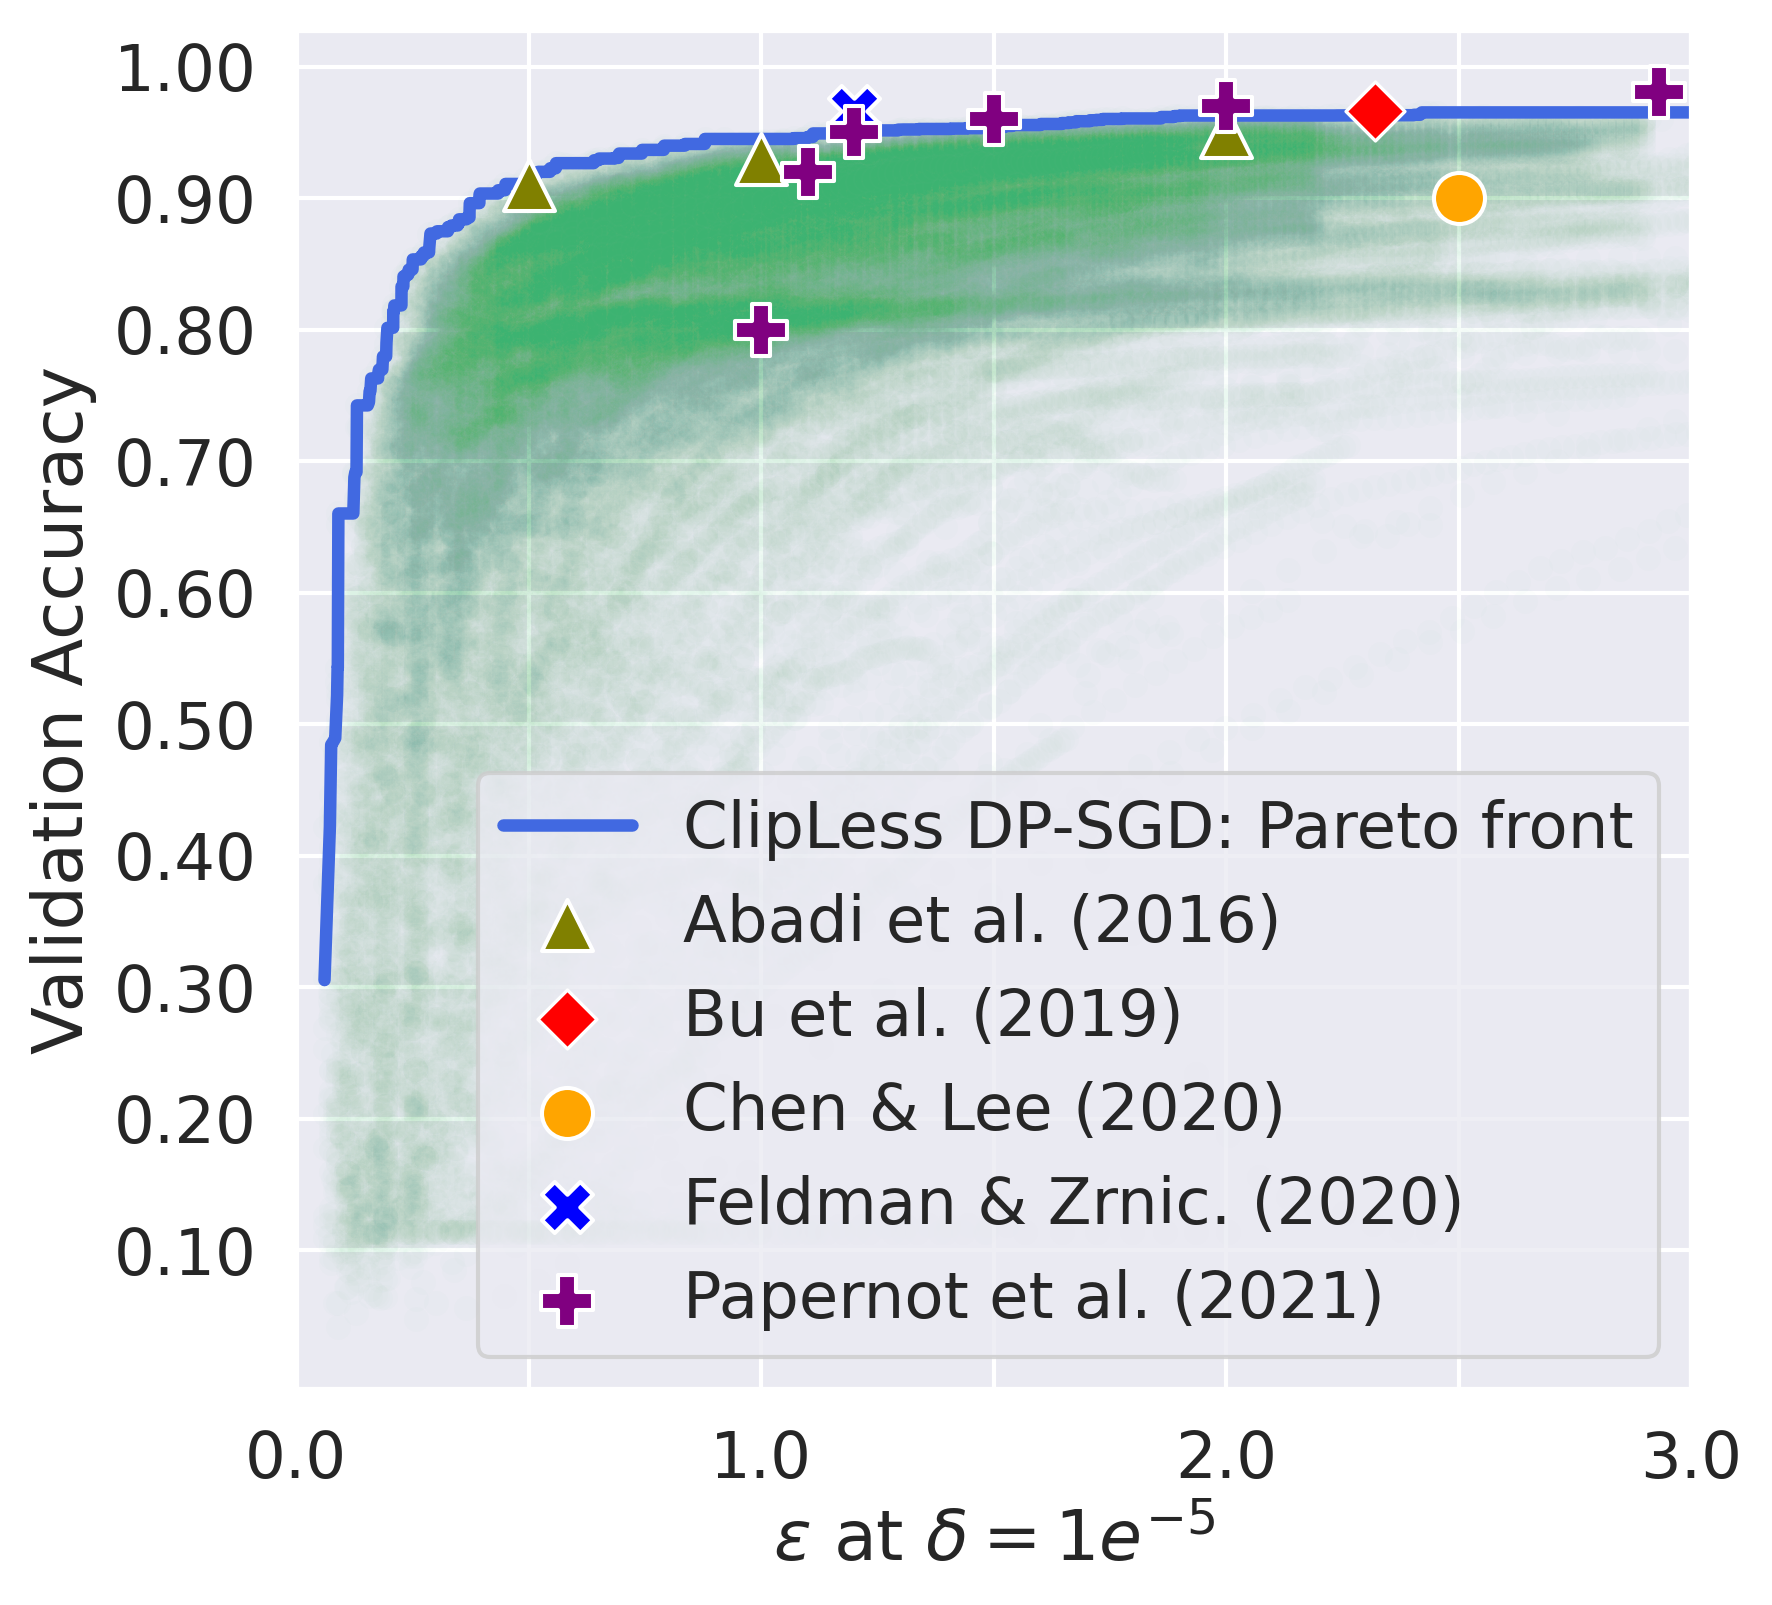
\includegraphics[width=\linewidth]{figures/mnist.png}
    \caption{\textbf{Pareto front on Mnist.} Each green dot corresponds to a (\textbf{val. acc}, $\epsilon$) pair from an epoch.}
    \label{fig:mnistmain}
  \end{subfigure}
}
\caption{\textbf{Comparison of the utility of DP-SGD and Clipless DP-SGD} on tabular and image data.}
\end{figure}

\textbf{Robustness and Privacy.} One of the most prominent advantage of Lipchitz networks is their ability to provide robustness certificates against adversarial attacks, and was the primary motivation for their development~\citep{szegedy2013,li2019preventing,fazlyab2019efficient}. For a $\ell$-Lipschitz classifier $f$, with predictions $\bar k\defeq\argmax_{k} f_k(x)$ the decision is invariant under perturbation of norms smaller than $\frac{1}{\ell\sqrt{2}}(f_{\bar k}(x)-\argmax_{i\neq \bar k}f_i(x))$. Therefore, for each perturbation radius $r$ we can measure the accuracy of the perturbed network, and we report these results in Fig.~\ref{fig:paretofrontrobust}. 
The computation of the certificates is straightforward, while methods applicable to conventional networks (like randomized smoothing~\citep{pmlr-v97-cohen19c} or interval propagation, see remark~\ref{remark:forwardbounds}), are expensive.  
This suggests that robust decisions and privacy are not necessarily antipodal objectives, contrary to what was observed in~\cite{song2019privacy}. The work of~\cite{wu2023augment} also study the link between certified robustness and privacy, albeit through the lens of adversarial training~\citep{zhang2019theoretically}. % of a pre-trained network.  

\begin{figure}%[hb]
    \centering
    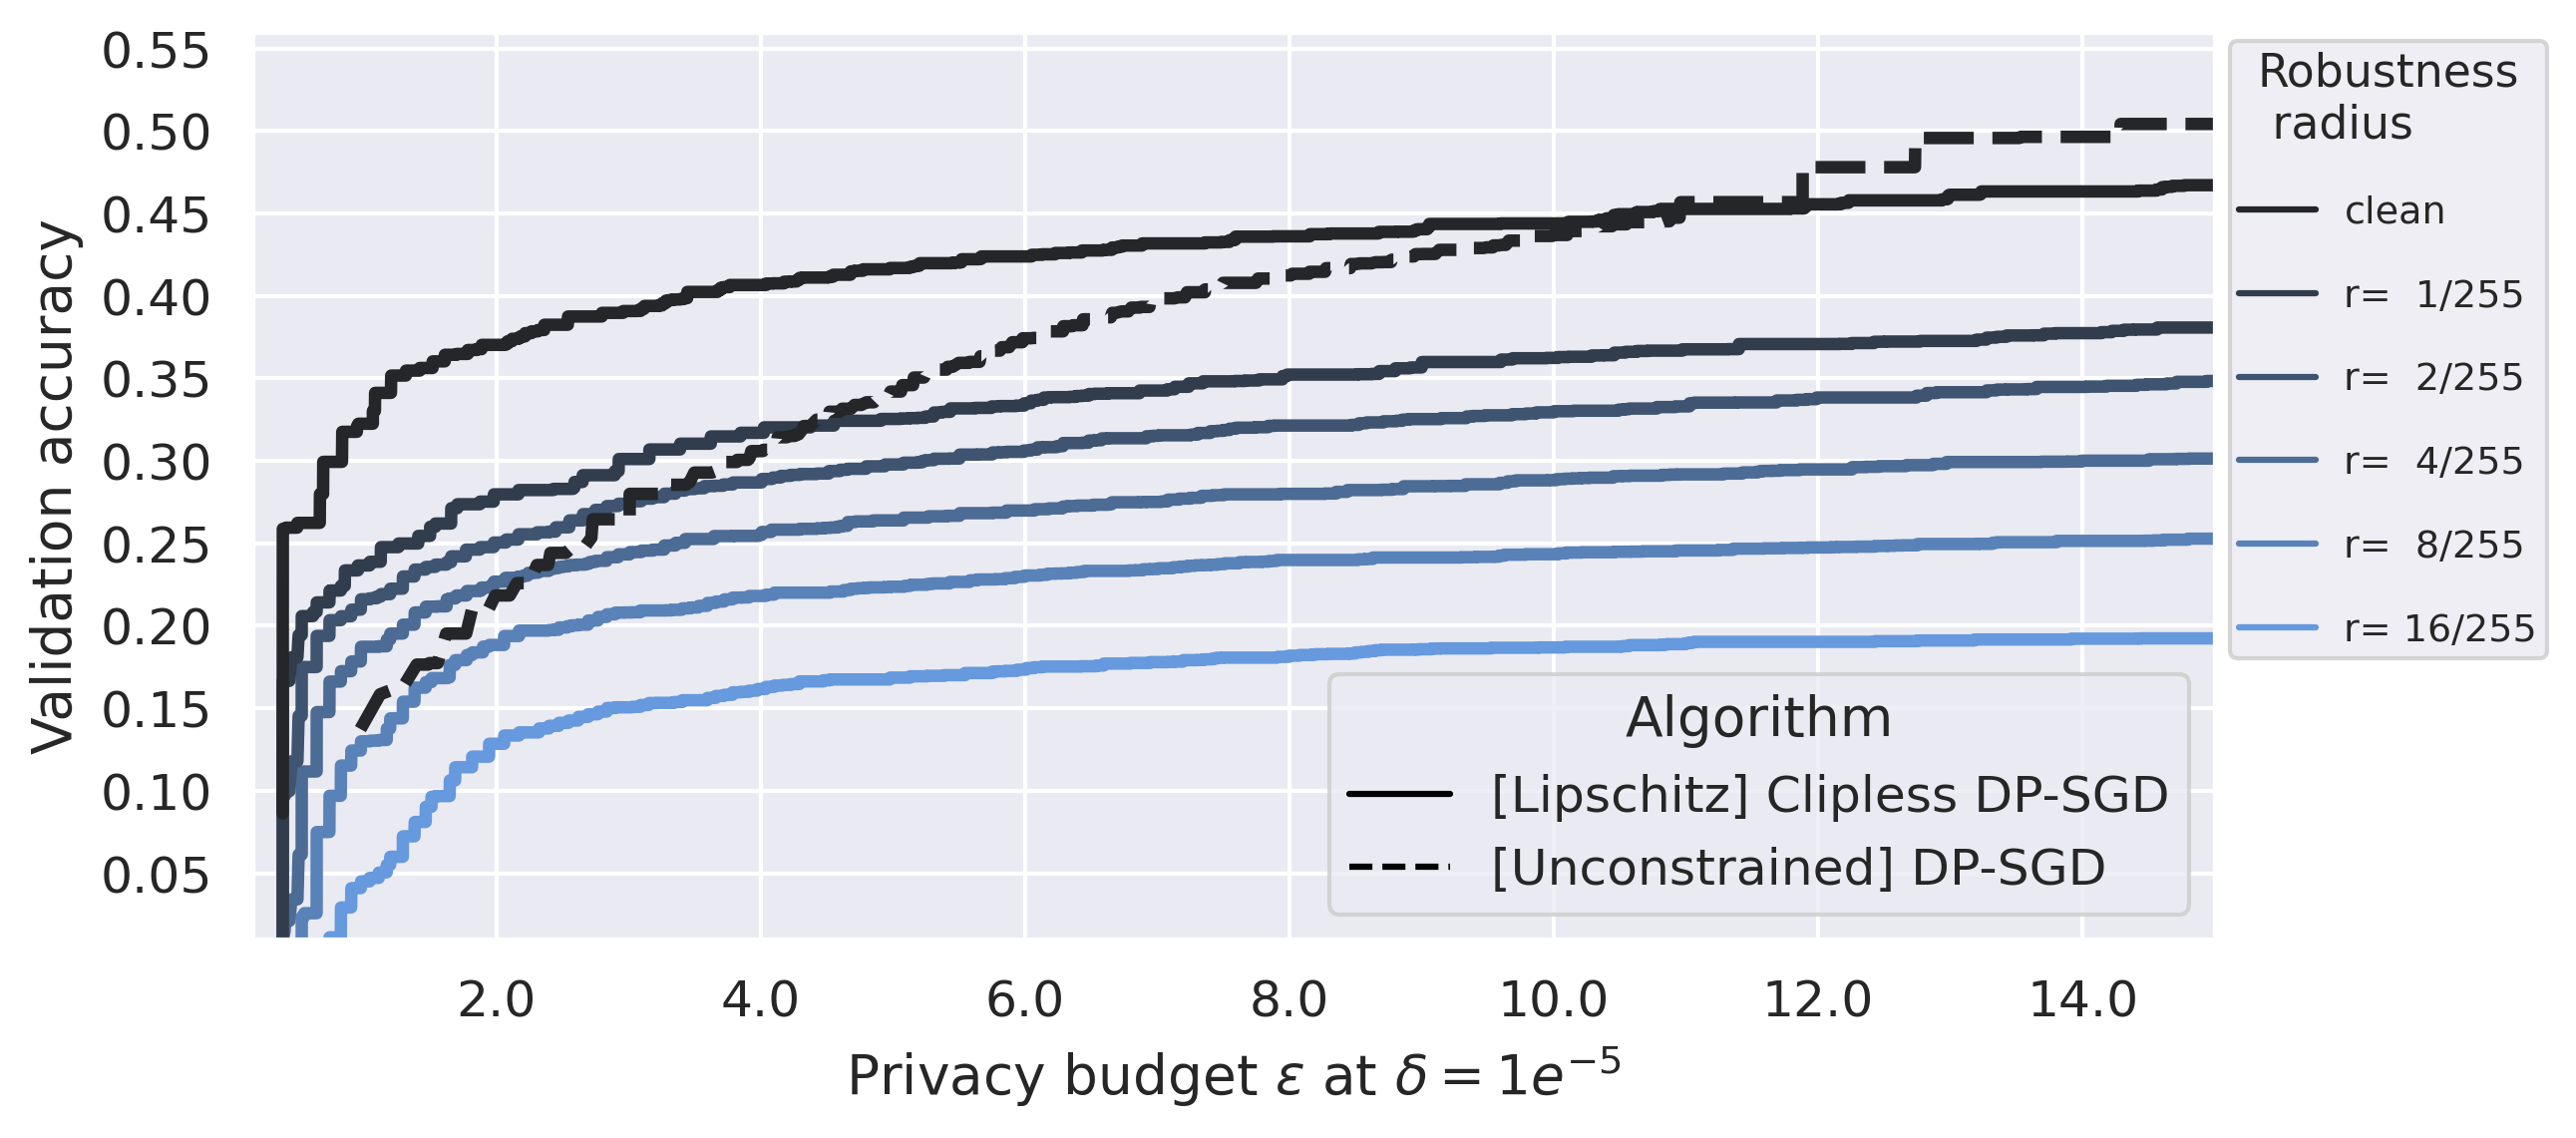
\includegraphics[width=0.9\textwidth]{figures/robustness_cifar10_VARIANTE.png}
    % \caption{\textbf{Our framework paints a clearer picture of the privacy/accuracy/robustness trade-off on Cifar-10.} We trained models in an "out of the box setting" (no pre-training, no data augmentation and no handcrafted features). For the Lipschitz network we report the robustness certificates at different radii, whereas a model without Lipschitz constraint cannot produce robustness certificates.}\label{fig:paretofrontrobust}
    \caption{\textbf{Privacy/accuracy/robustness trade-off on Cifar-10:} We report the pareto front of robustness certificates at different radii $r$ for Lipschitz constrained networks, while unconstrained networks cannot produce robustness certificates. Models are trained in an "out of the box setting": no pre-training, no data augmentation and no handcrafted features. \rebuttal{To ensure a fair comparison between algorithms, we perform 30 repetitions with a Bayesian optimizer to select the best hyper-parameters.}}\label{fig:paretofrontrobust}
\end{figure}

\subsection{Speed and memory consumption}\label{sec:batchspeed}

 We benchmarked the median runtime per batch of vanilla DP-SGD against the one of Clipless DP-SGD, on a CNN architecture and its Lipschitz equivalent respectively. The experiment was run on a GPU with 48GB video memory. We compare against the implementation of \lstinline[basicstyle=\ttfamily, backgroundcolor=\color{gray!20}]{tf_privacy}, \lstinline[basicstyle=\ttfamily, backgroundcolor=\color{gray!20}]{opacus} and \lstinline[basicstyle=\ttfamily, backgroundcolor=\color{gray!20}]{optax}. In order to allow a fair comparison, when evaluating Opacus, we reported the runtime with respect to the logical batch size, while capping the physical batch size to avoid Out Of Memory error (OOM). 
 \begin{wrapfigure}{r}{0.5\textwidth}
    \vspace{-5mm}
    \center
    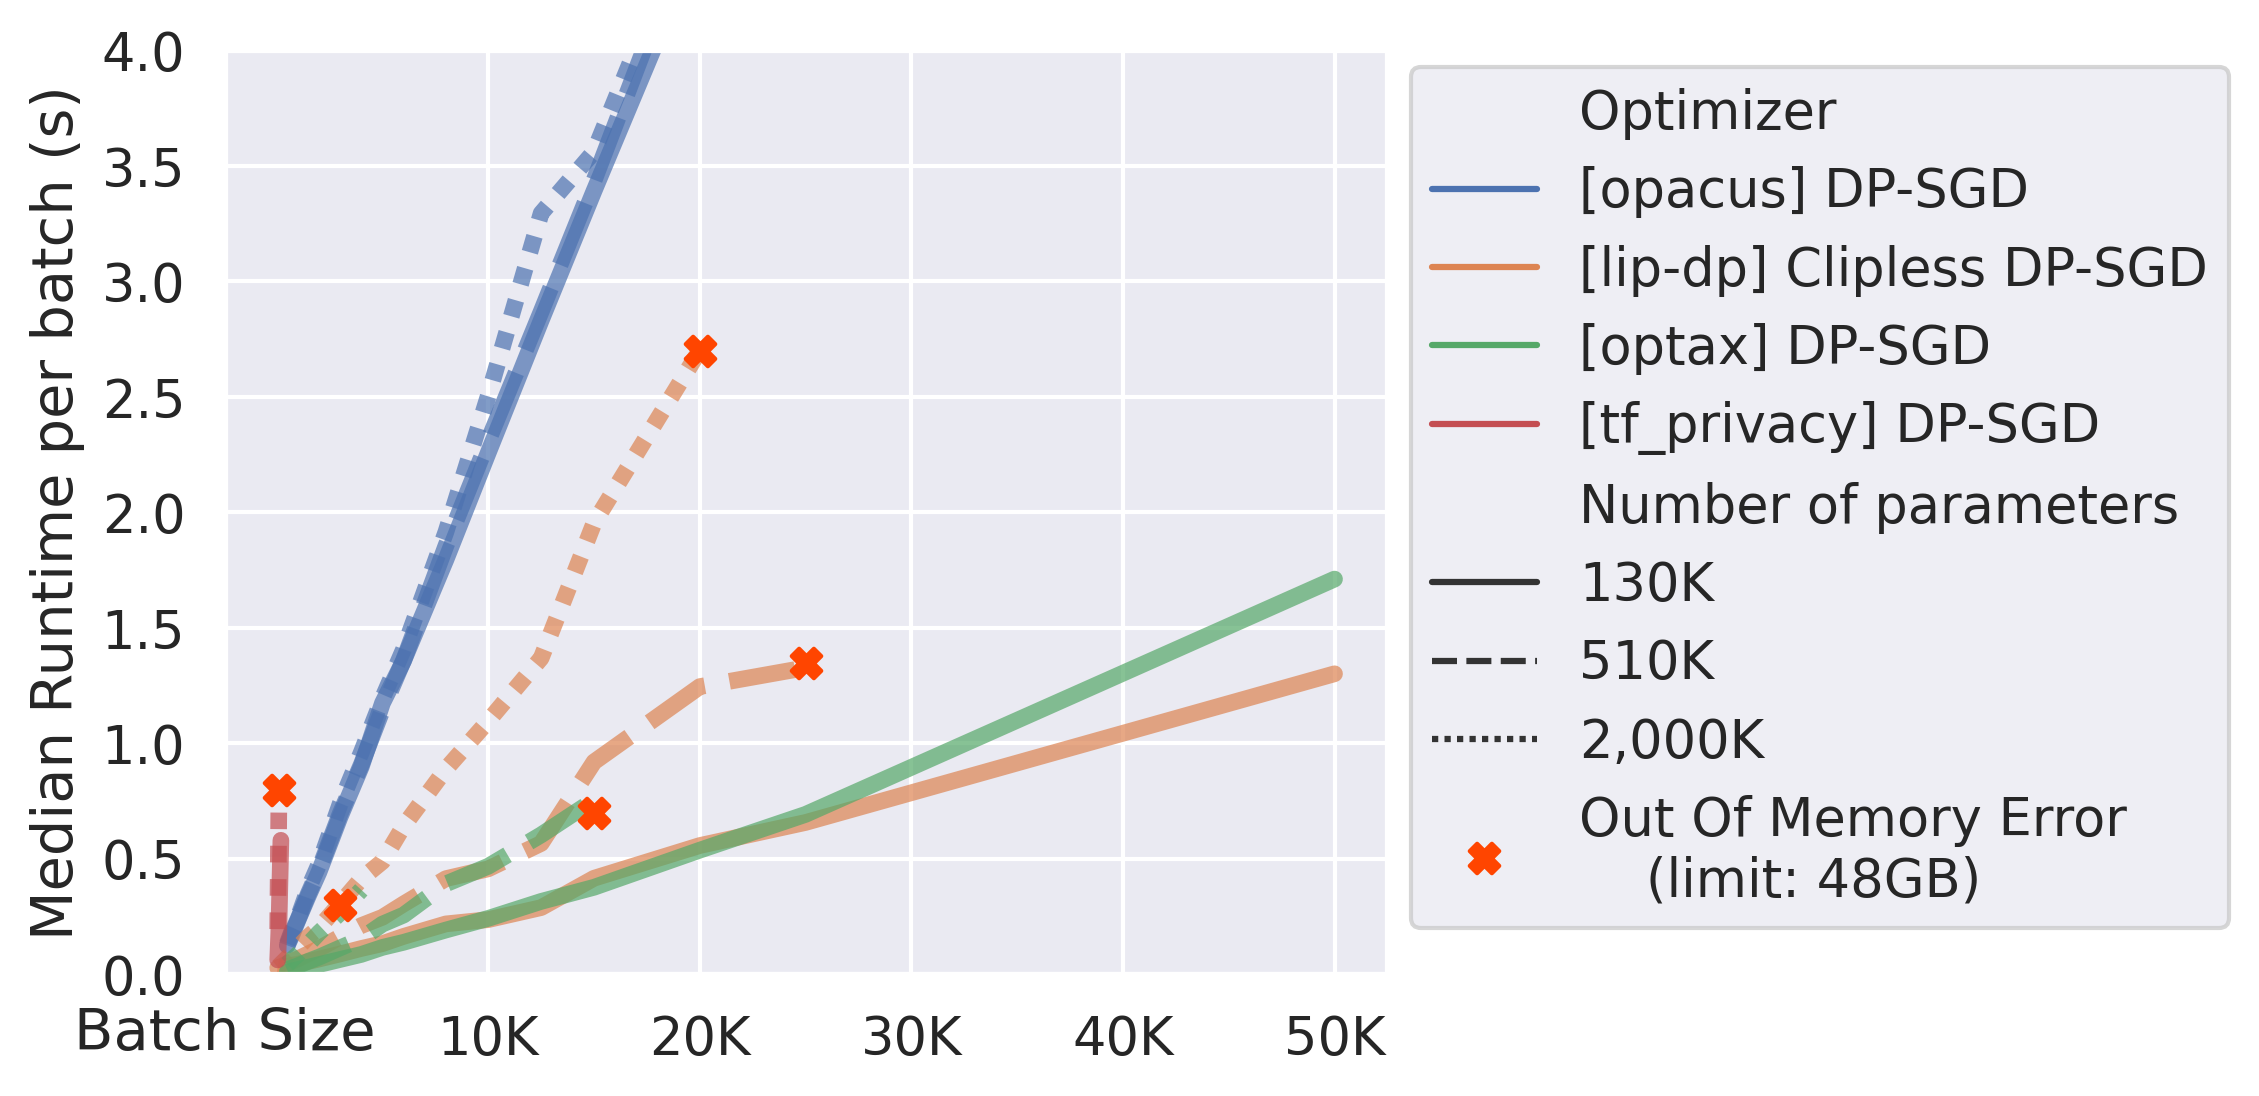
\includegraphics[width=0.5\textwidth]{figures/all_speed_curves.png}
    \caption{\textbf{Our approach outperforms concurrent frameworks in terms of runtime and memory:} we trained CNNs (ranging from 130K to 2M parameters) on CIFAR-10, and report the median batch processing time (including noise, and constraints application~$\Pi$ or gradient clipping).}
    \label{fig:runtime}
    \vspace{-5mm}
\end{wrapfigure}
% Although our library does not implement logical batching yet, it is fully compatible with this feature.   
% The study of~\cite{sander2022tan} suggests that utility decrease with batch size when the Total Amount of Noise $\frac{\sigma}{p}\sqrt{\frac{2}{S}}$ is kept constant. However our experiments on Lipschitz network tend to demonstrate that higher batch size typically help: indeed 

An advantage of the projection $\Pi$ over per-sample gradient clipping is that its cost is independent of the batch size. Fig~\ref{fig:runtime} validates that our method scales much better than vanilla DP-SGD, and is compatible with large batch sizes. It offers several advantages: firstly, a larger batch size contributes to a decrease of the sensitivity $\Delta\propto 1/b$, which diminishes the ratio between noise and gradient norm. Secondly, as the batch size~$b$ increases, the variance decreases at the parametric rate $\BigO(\sqrt{b})$ (as demonstrated in appendix~\ref{app:vargrad}), aligning with expectations. This observation does not apply to DP-SGD: clipping biases the direction of the average gradient, as noticed by~\cite{chen2020understanding}.  
